%%%%%%%%%%%%%%%%%%%%%%%%%%%%%%%%%%%%%%%%%
% Structured General Purpose Assignment
% LaTeX Template
%
%
%%%%%%%%%%%%%%%%%%%%%%%%%%%%%%%%%%%%%%%%%

%----------------------------------------------------------------------------------------
%	PACKAGES AND OTHER DOCUMENT CONFIGURATIONS
%----------------------------------------------------------------------------------------

\documentclass[11pt,a4paper,titlepage]{article}



\usepackage{amsfonts}
\usepackage{amssymb}
\usepackage{amsmath}

%\usepackage{fouriernc}
%\usepackage{pxfonts}
\usepackage[charter]{mathdesign}
\usepackage[no-math]{fontspec}
%\usepackage{polyglossia}
\usepackage{fancyhdr}
\usepackage{lastpage}
\usepackage{extramarks}
\usepackage{graphicx}
\usepackage{xltxtra}
\usepackage{makeidx}
\usepackage{enumerate}
\usepackage{caption}
%\usepackage{algorithm}
%\usepackage{algorithmic}
\usepackage[hidelinks]{hyperref}
\usepackage{grffile}
\usepackage{adjustbox}
\usepackage{dirtree}
\usepackage{xfrac}
\usepackage{wrapfig}
\usepackage{subcaption}
\usepackage{pgfplots}
\usepackage{tikz}
\usepackage{tikzscale}
\usetikzlibrary{plotmarks}


\setmainfont[
UprightFont = *,
ItalicFont = *Italics,
SlantedFont = *Italics,
BoldFont = *sb,               
BoldItalicFont = *sbi,
BoldSlantedFont = *sbi,       
SmallCapsFont = *SmallCaps
]{Kerkis}

\newfontfamily{\greekfont}[
UprightFont = *,
ItalicFont = *Italics,
SlantedFont = *Italics,
BoldFont = *sb,               
BoldItalicFont = *sbi,
BoldSlantedFont = *sbi,       
SmallCapsFont = *SmallCaps
]{Kerkis}



% Margins
\topmargin=-0.45in
\evensidemargin=0in
\oddsidemargin=0in
\textwidth=6.5in
\textheight=9.15in
\headsep=0.25in 

\linespread{1.1} % Line spacing

% Set up the header and footer
\pagestyle{fancy}
\lhead{} % Top left header
\chead{\hmwkClass\ - \hmwkTitle} % Top center header
\rhead{\firstxmark} % Top right header
\lfoot{\lastxmark} % Bottom left footer
\cfoot{} % Bottom center footer
\rfoot{Σελίδα\ \thepage\ από\ \pageref{LastPage}} % Bottom right footer
\renewcommand\headrulewidth{0.4pt} % Size of the header rule
\renewcommand\footrulewidth{0.4pt} % Size of the footer rule

\setlength\parindent{0pt} % Removes all indentation from paragraphs

%----------------------------------------------------------------------------------------
%	DOCUMENT STRUCTURE COMMANDS
%	Skip this unless you know what you're doing
%----------------------------------------------------------------------------------------

\setcounter{secnumdepth}{0}
\setcounter{tocdepth}{1}

\DTsetlength{0.3em}{1.2em}{0.2em}{0.4pt}{0pt}
\newcommand*\rfrac[2]{{}^{#1}\!/_{#2}}

%----------------------------------------------------------------------------------------
%	LOCALIZATION
%----------------------------------------------------------------------------------------

\renewcommand\figurename{Σχήμα}
\renewcommand\contentsname{Περιεχόμενα}
\renewcommand\indexname{Ευρετήριο}
\renewcommand\tablename{Πίνακας}
\renewcommand\appendixname{Παράρτημα}

%----------------------------------------------------------------------------------------
%	NAME AND CLASS SECTION
%----------------------------------------------------------------------------------------

\newcommand{\hmwkTitle}{Εργασία 2} % Assignment title
\newcommand{\hmwkClass}{Παράλληλα \& Διανεμημένα Συστήματα} % Course/class
\newcommand{\hmwkAuthorName}{Δημανίδης Ιωάννης} % Your name
\newcommand{\hmwkAuthorAEM}{8358} % Your ΑΕΜ

%----------------------------------------------------------------------------------------
%	MISC OPTIONS
%----------------------------------------------------------------------------------------

\graphicspath{{./figures/}}
\newcommand{\norm}[1]{\left\lVert#1\right\rVert}
\makeatletter
\newcommand{\xRightarrow}[2][]{\ext@arrow 0359\Rightarrowfill@{#1}{#2}}
\makeatother
\pgfplotsset{compat=newest}
\pgfplotsset{plot coordinates/math parser=false}
\newlength\figureheight
\newlength\figurewidth

%----------------------------------------------------------------------------------------
%	TITLE PAGE
%----------------------------------------------------------------------------------------

\title{
	\vspace{5cm}
	\huge{\textbf{\hmwkClass}}\\
	\vspace{9pt}
	\LARGE{\hmwkTitle}\\
	\vspace{7cm}
}

\author{\textbf{\hmwkAuthorName\ - \hmwkAuthorAEM}
		\vspace{0.5em}\\
		\textbf{Ζήσης Κωνσταντίνος\ - 7682}
		\vspace{0.5em}\\
		\textbf{Αθανασιάδης Ιωάννης\ - 7647}}
\date{} % Insert date here if you want it to appear below your name

%----------------------------------------------------------------------------------------

\begin{document}
	
	\maketitle
	
	%----------------------------------------------------------------------------------------
	%	TABLE OF CONTENTS
	%----------------------------------------------------------------------------------------
	
	%\setcounter{tocdepth}{1} % Uncomment this line if you don't want subsections listed in the ToC
	
	%\newpage
%	\tableofcontents
%	\clearpage
	%\newpage
	
	
	%----------------------------------------------------------------------------------------
	%	Document
	%----------------------------------------------------------------------------------------
	\section{Γενικά}
	Καλούμαστε να υλοποιήσουμε κατανεμημένο KNN αλγόριθμο με τη χρήση του πρωτοκόλλου MPI μέσα σε τρισδιάστατο μοναδιαίο κύβο. Έχουμε $N_Q$ ομοιόμορφα κατανεμημένα σημεία $q$ για τα οποία θέλουμε να βρούμε τον κοντινότερο γείτονα ανάμεσα σε $N_C$ σημεία $c$ κατα-κερματίζοντας το χώρο σε ένα grid $n\cdot m \cdot k$ κουτιών. Ορίζουμε λοιπόν το ακόλουθο project structure:\\
	
	\begin{wrapfigure}{r}{0.4\textwidth}
		\begin{minipage}[t]{0.4\textwidth}
			\dirtree{%
				.1 trunk/.
				.2 bin/.
				.3 mpi-knn.
				.2 build/.
				.3 mpi-knn.o.
				.3 vector.o.
				.2 include/.
				.3 mpi-knn.h.
				.3 vector.h.
				.2 src/.
				.3 mpi-knn.c.
				.3 vector.c.
			    .2 README.md.
			    .2 makefile.
			    .2 mpi-knn.pbs.
				.2 run\_all.sh.
			}
		\end{minipage}
		\caption{Project Structure}			
	\end{wrapfigure}
	 
	Στον φάκελο \verb|bin/| έχουμε το εκτελέσιμο αρχείο \verb|mpi-knn| το οποίο δέχεται 4 ορίσματα: $n_q, n_c, nmk, v$ και εκτελεί την αναζήτηση ΚΝΝ για κάθε σημέιο $q$ από $N_Q = 2^{n_q}$ ανάμεσα σε 
	$N_C = 2^{n_c}$ σημεία $c$, σε πλέγμα $nmk$ στοιχείων. Η σημαία $v$ δηλώνει το αν θα γίνει σειριακή επαλήθευση των αποτελεσμάτων.\footnote{Ο χρήστης έχει την δυνατότητα να μην επαληθεύσει σειριακά τα αποτελέσματα, καθώς για μεγάλα πλήθη σημείων η διαδικασία αυτή μπορεί να προβεί πολύ χρονοβόρα.} Επιπλέον, η default συμπεριφορά του προγράμματος είναι να μην εκτυπώνει ως έξοδο τα ζεύγη γειτόνων $q,c$, καθώς τα αρχεία εξόδου μπορούν να έχουν μεγάλο μέγεθος και να μην είναι εύκολα διαχειρίσιμα.
	Στον κατάλογο  \verb|build/| βρίσκονται τα compiled object files από το κάθε αρχέιο, τα οποία γίνονται αργότερα link μεταξύ τους και των βιβλιοθηκών του συστήματος για να παράξουν το εκτελέσιμο \verb|mpi-knn|. Στο φάκελο \verb|include/| βρίσκονται τα header files για το κάθε αρχέιο κώδικα,  τα οποία αρχεία βρίσκονται στο directory \verb|src/|.\\
	
	Επιπλέον υπάρχουν τα αρχεία \verb|README.md|, \verb|makefile|, \verb|mpi-knn.pbs|, \verb|run_all.sh|, από τα οποία το πρώτο αποτελεί ένα συνοπτικό οδηγό χρήσης του προγράμματος, ενώ το αρχείο \verb|makefile| περιέχει οδηγίες για την εντολή make. Το αρχείο \verb|mpi-knn.pbs|, περιέχει directives για το Sun Grid Engine που χρησιμοποιεί το hellasgrid, ενώ το \verb|run_all.sh| αποτελεί ένα bash script το οποίο τρέχει όλους τους πιθανούς συνδυασμούς $N_Q, N_C, n \cdot m \cdot k$ που ζητούνται.\\
	
	Τέλος, να σημειωθεί ότι χρησιμοποιήθηκε η έκδοση 4.4.7 του \verb|gcc| με optimization level \verb|-O3|. Η διαδικασία για την επαλήθευση των αποτελεσμάτων είναι η εξής: αρχικά πρέπει το πρόγραμμα να μεταγλωττιστεί με την σημαία \verb|VRB = 1| μέσα στο source file \verb|mpi-knn.c|, ώστε να τυπώνει τα ζεύγη γείτόνων $q, c$. Έπειτα πρέπει να καταγραφεί η έξοδος του προγράμματος, και να συγκριθούν τα ζεύγη γειτνίασης της υλοποίησής μας με τα ζεύγη της σειριακής naive υλοποίησης με τη χρήση κάποιου εργαλείου όπως το \verb|diff|. Ο λόγος που δεν ενσωματώθηκε η δυνατότητα αυτή στο πρόγραμμά μας είναι χάριν απλότητας κώδικα και εξοικονόμησης μνήμης, γιατί θα έπρεπε κάθε instance του προγράμματος να κρατάει μια δομή με το κάθε ζεύγος και μετά να τα στέλνει στο master process για επαλήθευση.
	
	\section{Παράλληλη Υλοποίηση}
	Αρχικά χωρίζουμε το μοναδιαίο κύβο σε 2 διακριτά grids ταυτόχρονα: ένα global grid $ n \cdot m \cdot k$ στοιχείων, και ένα πλέγμα το οποίο προκύπτει από τον αριθμό των διεργασιών που τρέχουν παράλληλα το πρόγραμμα, διαστάσεων $w \cdot h \cdot d$, με $w \leq h \leq d$. Αν λοιπόν ο αριθμός των διεργασιών είναι $2^p, p \in [0, 7]$ τότε το global και το process grid έχουν ως εξής:
	
	\begin{minipage}[l]{0.6\textwidth}
		\begin{align*}
			& \text{If } n \cdot m \cdot k \bmod 3 = 0 \Rightarrow \begin{cases} n = 2^{n \cdot m \cdot k/3}\\ m = 2^{n \cdot m \cdot k/3}\\ k = 2^{n \cdot m \cdot k/3}\end{cases}\\
			& \text{If } n \cdot m \cdot k \bmod 3 = 1 \Rightarrow \begin{cases} n = 2^{\lfloor n \cdot m \cdot k/3 \rfloor}\\ m = 2^{\lfloor n \cdot m \cdot k/3 \rfloor}\\ k = 2^{\lfloor n \cdot m \cdot k/3 \rfloor + 1}\end{cases}\\
			& \text{If } n \cdot m \cdot k \bmod 3 = 2 \Rightarrow \begin{cases} n = 2^{\lfloor n \cdot m \cdot k/3 \rfloor}\\ m = 2^{\lfloor n \cdot m \cdot k/3 \rfloor + 1}\\ k = 2^{\lfloor n \cdot m \cdot k/3 \rfloor + 1}\end{cases}
		\end{align*}
	\end{minipage}
	\begin{minipage}[r]{0.4\textwidth}
		\begin{align*}
			& \text{If } p \bmod 3 = 0 \Rightarrow \begin{cases} w = 2^{p/3}\\ h = 2^{p/3}\\ d = 2^{p/3}\end{cases}\\
			& \text{If } p \bmod 3 = 1 \Rightarrow \begin{cases} w = 2^{\lfloor p/3 \rfloor}\\ h = 2^{\lfloor p/3 \rfloor}\\ d = 2^{\lfloor p/3 \rfloor + 1}\end{cases}\\
			& \text{If } p \bmod 3 = 2 \Rightarrow \begin{cases} w = 2^{\lfloor p/3 \rfloor}\\ h = 2^{\lfloor p/3 \rfloor + 1}\\ d = 2^{\lfloor p/3 \rfloor + 1}\end{cases}
		\end{align*}
	\end{minipage}\\
	
	Οι σταθερές $n, m, k, w, h, d$ όπως φαίνεται και από τους άνω τύπους, επιλέγονται έτσι ώστε να τα κο		 		υτιά του εκάστοτε πλέγματος να είναι ένα ορθογώνιο παραλληλεπίπεδο με τις όσες περισσότερες ίσες ακμές γίνεται, στην ιδανική περίπτωση ένα κύβο. Προσπαθώντας να πετύχουμε συμμετρία και στις τρεις διαστάσεις, αυξάνουμε την αποδοτικότητα του αλγο-ρίθμου. Κάθε στοιχείο του process grid αποτελεί μια διεργασία και μέσω του πλέγματος αυτού μπορούμε εύκολα να κατανείμουμε περιοχές του χώρου σε αυτές. Γενικά, το global grid θα έχει μεγαλύτερη ανάλυση του χώρου από το πλέγμα των διεργασιών, δηλαδή θα ισχύει $n \geq w, m \geq h, k \geq d$. Συνεπώς, σε κάθε process θα ανήκει ένα διακριτό ενιαίο συνεχό-μενο υποσύνολο  του γενικού πλέγματος. Τα πλέγματα αυτά παρόλο που ανήκουν στις τρεις διαστάσεις, τα μετατρέπουμε σε μονοδιάστατους πίνακες χρησιμοποιώντας flat indexing. Έτσι, γνωρίζοντας τις τρισδιάστατες συντεταγμένες $x,y,z$ ενός κουτιού του γενικού πλέγματος μπορούμε να βρούμε το flat array index του με τον τύπο
	\begin{equation}
		\mathrm{index_g} = x + y\cdot n + z \cdot n\cdot m
	\end{equation}
	ενώ για το πλέγμα διεργασιών ο αντίστοιχος τύπος είναι
	\begin{equation} \label{eq:2}
		\mathrm{index_p} = x + y\cdot w + z \cdot w\cdot h
	\end{equation}
	όπου το index σε αυτήν την περίπτωση αντιστοιχεί στο rank της εκάστοτε διεργασίας. Για την αντιστροφή διαδικασία, όπου έχουμε το δείκτη του μονοδιάστατου πίνακα και θέλουμε να βρούμε τις τρισδιάστατες συντεταγμένες στο γενικό πλέγμα, έχουμε τους τύπους
	\begin{align}
		x_g &= \mathrm{index} \bmod n\\
		y_g &= \left(\left(\mathrm{index} - x_g\right)/n\right) \bmod m\\
 		z_g &= \left(\left(\mathrm{index} - x_g\right)/n - y_g\right) / m
	\end{align}
	και αντίστοιχα αν έχουμε το δείκτη για το πλέγμα διεργασιών, οι τρισδιάστατες συντεταγμένες προκύπτουν από τους τύπους
 	\begin{align}
	 	x_p &= \mathrm{index} \bmod w\\
	 	y_p &= \left(\left(\mathrm{index} - x_p\right)/w\right) \bmod h\\
	 	z_p &= \left(\left(\mathrm{index} - x_p\right)/w - y_p\right) / h
 	\end{align}\\[-2em]
 	
 	Έπειτα, δημιουργούμε $N_Q$ τυχαία τρισδιάστατα σημεία $q$ κατανεμημένα σε $2^p$ διεργασίες, και τα ταξινομούμε μέσα στο πλέγμα των διεργασιών ανάλογα με τις συντεταγμένες τους. Μάλιστα, έχοντας τις τρισδιάστατες συντεταγμένες $q_x, q_y, q_z$ μέσα στο μοναδιαίο κύβο, μπο-ρούμε να εξάγουμε το υποκουτί του πλέγματος διεργασιών μέσα στο οποίο ανήκει μέσα από τους τύπους
 	\begin{align}
	 	q_{x_p} &= \lfloor q_x \cdot w \rfloor\\
	 	q_{x_p} &= \lfloor q_y \cdot h \rfloor\\
	 	q_{x_p} &= \lfloor q_z \cdot d \rfloor
 	\end{align}
 	όπου $q_{x_p}$ εκφράζει την $x$-συντεταγμένη στο πλέγμα των διεργασιών του σημείου $q$. Γνωρί-ζοντας σε πιο κουτί του process grid ανήκει ένα σημείο $q$, αυτομάτως γνωρίζουμε και σε ποια διεργασία ανήκει. Όταν ένα process δημιουργεί ένα σημείο το οποίο ανήκει σε άλλη διεργασία, το αποθηκεύει προσωρινά σε ένα πίνακα από $2^p$ vectors, ανάλογα με το rank της. Προφανώς κάθε διάνυσμα κρατάει όλα τα σημεία $q$ που παράχθηκαν από την τρέχουσα διεργασία και προορίζονται για τη διεργασία με rank τον δείκτη του vector στον πίνακα. Εφόσον όλα τα processes τελειώσουν με τη δημιουργία των σημείων $q$, ξεκινάει η διαδικασία του διαμοιρασμού τους. Η κάθε διεργασία στέλνει διαδοχικά σε όλες τις υπόλοιπες τα ανάλογα διανύσματα με τα σημεία $q$, και με το που τελειώσει η διαδικασία αυτή, το κάθε process αρχίζει να ταξινομεί τα ληφθέντα σημεία ανάμεσα σε $(n/w)\cdot (m/h)\cdot (k/d)$ κουτιά που ανήκουν στο εσωτερικό υποσύνολο του γενικού πλέγματος της κάθε διεργασίας, για το οποίο χρησιμοποιούνται σχετικές συντεταγμένες. Πιο συγκεκριμένα, μια διεργασία ταξινομεί ένα σημείο $q$ στο δικό της τμήμα του γενικού πλέγματος με την χρήση των εξισώσεων
 	\begin{align}
	 	q_{x_g^{(i)}} &= \lfloor q_x \cdot n \rfloor -  {x_p^{(i)}}\cdot n/w \label{eq:12}\\
	 	q_{y_g^{(i)}} &= \lfloor q_y \cdot m \rfloor -  {y_p^{(i)}}\cdot m/h \label{eq:13}\\
	 	q_{z_g^{(i)}} &= \lfloor q_z \cdot k \rfloor -  {z_p^{(i)}}\cdot k/d \label{eq:14}
 	\end{align}
 	όπου $i$ το rank της διεργασίας. Δηλαδή, το ${x_p^{(i)}}$ εκφράζει τη $x$-συντεταγμένη του rank της $i$-οστής διεργασίας και το $q_{x_g^{(i)}}$ εκφράζει την $x$-συντεταγμένη στο υποσύνολο του γενικού πλέγματος που ανάγεται στην $i$-οστή διεργασία για το σημείο $q$. Όπως φαίνεται και από τους άνω τύπους, κανονικοποιούμε τις διαστάσεις του γενικού πλέγματος μέσα στα όρια του πλέγματος της κάθε διεργασίας, και έτσι ο μονοδιάστατος δείκτης πλέγματος είναι:
	\begin{equation}
	 	q_{\mathrm{index}_g^{(i)}} = q_{x_g^{(i)}} + q_{y_g^{(i)}} \cdot n/w + q_{z_g^{(i)}}\cdot n/w \cdot m/h 
	\end{equation}\\[-2em]
 	
 	Έπειτα ακολουθεί η δημιουργία του συνόλου $C$, το οποίο περιέχει $N_C$ τυχαία τρισδιάστατα σημεία $c$, κατανεμημένα σε $2^p$ διεργασίες. Όμως, εδώ τίθεται ένα ζήτημα. Κανονικά ο αλγόριθμος θα πρέπει για κάθε σημείο $q$, να βρίσκει σε πιο κουτί του γενικού πλέγματος ανήκει και να ψάχνει και σε αυτό και στα εφαπτόμενα γειτονικά του για τον κοντινότερο γείτονα $c$, καθώς δεν είναι δεδομένο ότι αυτός θα βρίσκεται στο ίδιο κουτί με το $q$. Βέβαια, το επιχείρημα αυτό μπορεί να επεκταθεί περαιτέρω και να πει κάνεις ότι δεν είναι απαραίτητο να ανήκει ούτε στα γειτονικά κουτιά, καθώς αυτά μπορεί να είναι κενά. Όμως, δεδομένου του πλήθους των σημείων, καθώς και του γεγονότος ότι τα σημεία ακολουθούν ομοιόμορφη τυχαία κατανομή, μπορούμε με μεγάλη βεβαιότητα να θεωρήσουμε πως αυτό το ενδεχόμενο είναι στατιστικώς απίθανο. Κάνοντας λοιπόν αυτήν την παραδοχή, το μόνο που χρειάζεται πλέον είναι να ελέγξουμε μόνο τα άμεσα γειτονικά κουτιά. Όμως, τα κουτιά του γενικού πλέγματος τα οποία είναι στα σύνορα του χώρου της εκάστοτε διεργασίας, θα βρίσκονται σε διαφορετικό process. Συνεπώς οι λύσεις είναι δύο: είτε να ζητάμε δυναμικά τα απαραίτητα κουτιά και το περιεχόμενο τους την ώρα της αναζήτησης του κοντινότερου γείτονα, είτε να στείλουμε μια φόρα όλα τα γειτονικά κουτιά του συνόρου του χώρου της κάθε διεργασίας. Η πρώτη λύση απορρίπτεται, καθώς αυτό θα εισήγαγε πολυπλοκότητα στον κώδικα, καθώς θα έπρεπε να υπάρχει ένα listening thread σε κάθε διεργασία, έτοιμο να απαντήσει σε κάθε πιθανό request δεδομένων, αλλά το κύριο μειονέκτημα αυτής της μεθόδου είναι ότι επειδή τα requests για κάθε κουτί θα ήταν ανεξάρτητα μεταξύ τους και απομονωμένα, θα εισάγαμε περιττό latency στις επικοινωνίες μας, και δεδομένου ότι οι επικοινωνίες μας θα είναι και δικτυακές, θα αυξανόταν ο χρόνος περάτωσης του αλγορίθμου κατά μεγάλο ποσοστό. Συνεπώς, για έναν αποδοτικό αλγόριθμο, θα πρέπει να βρούμε ένα ντετερμινιστικό τρόπο να στέλνουμε ahead-of-time όσα κουτιά είναι πιθανό να χρειαστεί μια διεργασία.\\
 	 	
 	Αρχικά λοιπόν, για κάθε σημείο $c$, βρίσκουμε σε ποιο κουτί του γενικού πλέγματος ανήκει μέσω των εξισώσεων:
 	\begin{align}
	 	c_{x_g} &= \lfloor c_x \cdot n \rfloor \label{eq:16}\\
	 	c_{y_g} &= \lfloor c_y \cdot m \rfloor \label{eq:17}\\
	 	c_{z_g} &= \lfloor c_z \cdot k \rfloor \label{eq:18}
 	\end{align}\\[-2em]
 	
 	Γνωρίζοντας τις συντεταγμένες του κουτιού του γενικού πλέγματος στο οποίο ανήκει το σημείο $c$, μπορούμε να βρούμε ποια κουτιά εφάπτονται σε αυτό. Όμως, η γειτνίαση είναι δυαδική ιδιότητα, δηλαδή όσα κουτιά γειτονεύουν στο κουτί $(c_{x_g}, c_{y_g}, c_{z_g})$, έχουν προφανώς ως κοινό γείτονα το κουτί αυτό. Συνεπώς, βρίσκοντας όλα τα γειτονικά κουτιά για κάθε σημείο $c$, αυτομάτως έχουμε ένα γειτονικό κουτί για τα κουτιά αυτά. Αν λοιπόν ένα γειτονεύων κουτί ανήκει σε διαφορετική διεργασία από την τρέχουσα, τότε στέλνουμε το σημείο $c$ και σε αυτήν, πέρα δηλαδή από τη διεργασία στην οποία ανήκει το κουτί $(c_{x_g}, c_{y_g}, c_{z_g})$. Τα εφαπτόμενα κουτιά του $(c_{x_g}, c_{y_g}, c_{z_g})$ στο χώρο του γενικού πλέγματος δίνονται από τους συνδυασμούς όλων των $(x,y,z)$ συντεταγμένων $\pm 1$. Έτσι, ορίζουμε τον τελεστή $\mathrm{Ne}\{\}$, o οποίος δοθέντων των συντεταγμένων ενός κουτιού, μας επιστρέφει τους άμεσους γείτονές του:
	\begin{equation}
		\mathrm{Ne}\{ (c_{x_g}, c_{y_g}, c_{z_g}) \} \triangleq \{c_{x_g} - 1, c_{x_g}, c_{x_g} + 1\} \times \{c_{y_g} - 1, c_{y_g}, c_{y_g} + 1\} \times \{c_{z_g} - 1, c_{z_g}, c_{z_g} + 1\} - \{(c_{x_g}, c_{y_g}, c_{z_g})\}
	\end{equation}
 	όπου $\times$ δηλώνει το καρτεσιανό γινόμενο μεταξύ δύο συνόλων. Χάριν συντομίας και ευκολίας γραφής μπορούμε να συμβολίζουμε το $\mathrm{Ne}\{ (c_{x_g}, c_{y_g}, c_{z_g}) \}$ ως $\mathrm{Ne}\{c\}$. 	
 	Προφανώς, ο τελεστής αυτός δε θα επιστρέφει το ίδιο το κουτί παρά μόνο τους γείτονές του. Για κάθε κουτί που ανήκει στο σύνολο  $\mathrm{Ne}\{c\}$, ελέγχουμε αν οι συντεταγμένες του είναι έγκυρες, γιατί μπορεί να βγούμε εκτός των ορίων του γενικού πλέγματος. Θεωρούμε το γειτνιάζων κουτί $(b_{x_g}^{(j)}, b_{y_g}^{(j)}, b_{z_g}^{(j)}) = \mathrm{Ne}\{c\}^{(j)}$, με $j \in \left[1, 26\right]$ να υποδείχνει το $j$-οστό στοιχείο του  συνόλου των γειτόνων. Δοθέντων λοιπόν των συντεταγμένων ενός κουτιού, μπορούμε να βρούμε σε ποια διεργασία ανήκει από τις εξισώσεις
 	\begin{align}
	 	b_{x_p}^{(j)} &= \lfloor b_{x_g}^{(j)} \cdot w/n \rfloor\\
	 	b_{y_p}^{(j)} &= \lfloor b_{y_g}^{(j)} \cdot h/m \rfloor\\
	 	b_{z_p}^{(j)} &= \lfloor b_{z_g}^{(j)} \cdot d/k \rfloor
 	\end{align}
 	όπου $b_{x_p}^{(j)}$ να αποτελεί τη $x$-συντεταγμένη της διεργασίας στην οποία υπάγεται το $j$-οστό στοιχείο του $\mathrm{Ne}\{c\}$. Για κάθε διαφορετικό συνδυασμό $(b_{x_g}^{(j)}, b_{y_g}^{(j)}, b_{z_g}^{(j)})$ μπορούμε εύκολα να εξάγουμε το rank της αντίστοιχης διεργασίας από την εξίσωση \eqref{eq:2}. Γνωρίζοντας πλέον το rank της διεργασίας μπορούμε να στείλουμε το σημείο $c$ σε αυτήν. Όπως και πριν έχουμε ένα πίνακα από vectors, με κάθε vector να έχει τα σημεία $c$ τα οποία υπάγονται στην διεργασία που έχει rank ίσο με το δείκτη του διανύσματος στον πίνακα.\\
 	
 	Έχοντας πλέον ταξινομήσει όλα τα στοιχεία $c$ ανάλογα με τον προορισμό τους, αρχίζει το δεύτερο κομμάτι των επικοινωνιών μεταξύ των διεργασιών, όπου στέλνουμε διαδοχικά σε κάθε μία διεργασία τα vectors με τα σημεία που υπάγονται σε αυτές. Να σημειωθεί ότι εδώ πλέον στέλνουμε πλέον περισσότερα κουτιά από πριν, καθώς κάθε διεργασία έχει και τα κουτιά που περιβάλλουν τα σύνορά της. Εδώ πλέον έχουμε $(n/w+2)\cdot(m/h + 2)\cdot(k/d + 2)$ κουτιά γενικού πλέγματος ανά διεργασία. Με το που λάβει μια διεργασία όλα τα σημεία που τις αντιστοιχούν, τοποθετούμε το κάθε σημείο στο αντίστοιχο του κουτί του γενικού πλέγματος σύμφωνα με τις εξισώσεις
	\begin{align}
	 	c_{x_g^{(i)}} &= c_{x_g} - {x_p^{(i)}}\cdot n/w + 1 \label{eq:23}\\
	 	c_{y_g^{(i)}} &= c_{y_g} - {y_p^{(i)}}\cdot m/h + 1 \label{eq:24}\\
	 	c_{z_g^{(i)}} &= c_{z_g} - {z_p^{(i)}}\cdot k/d + 1 \label{eq:25}
 	\end{align}
 	όπου $c_{x_g}, c_{y_g}, c_{z_g}$ οι συντεταγμένες των κουτιών γενικού πλέγματος που προκύπτουν από τις εξισώσεις \eqref{eq:16}-\eqref{eq:18}, και $c_{x_g^{(i)}}$ να αποτελεί τη $x$-συντεταγμένη του γενικού πλέγματος της $i$-οστής διεργασίας  για το σημείο $c$, ενώ το $x_p^{(i)}$ συμβολίζει τη $x$-συντεταγμένη του rank της $i$-οστής διεργασίας. Επειδή όπως προαναφέρθηκε, έχουμε $(n/w+2)\cdot(m/h + 2)\cdot(k/d + 2)$ κουτιά ανά διεργασία, σε αντίθεση με πριν που είχαμε μονάχα $(n/w)\cdot(m/h)\cdot(k/d)$, έχουμε ένα offset το οποίο διορθώνουμε προσθέτοντας $1$ στις συντεταγμένες και των τριών διαστάσεων, καθώς η αρίθμηση των πινάκων μας ξεκινάει μια θέση νωρίτερα. Να σημειωθεί ότι χρησιμοποιούμε το δείκτη ${x_p^{(i)}}$, γιατί αναφερόμαστε στην τρέχουσα διεργασία και όχι στην διεργασία στην οποία ανήκει το σημείο $c$. Σε αντίθεση με τις εξισώσεις \eqref{eq:12}-\eqref{eq:14} όπου η τρέχουσα διεργασία ταυτίζονταν με την διεργασία στην οποία άνηκε το σημείο $q$, εδώ αποτελούν δύο διαφορετικές έννοιες, καθώς η κάθε διεργασία περιλαμβάνει και σημεία $c$ που κανονικά δεν της ανήκουν, αλλά βρίσκονται στο σύνορο της με μια άλλη διεργασία.\\
 	
 	Πλέον, η κάθε διεργασία έχει λάβει και έχει ταξινομήσει τα υποσύνολα των $Q, C$ που υπάγο-νται σε αυτήν και μπορεί να ξεκινήσει η αναζήτηση του κοντινότερου γείτονα. Έτσι λοιπόν για κάθε σημείο $q$ βρίσκουμε το κουτί του υποσυνόλου του γενικού πλέγματος της $i$-οστής διεργασίας στο οποίο ανήκει μέσω των εξισώσεων \eqref{eq:12}-\eqref{eq:14} και για να τις ανάγουμε στα αντίστοιχα κουτιά του $C$ συνόλου προσθέτουμε 1, όπως κάναμε και στις εξισώσεις \eqref{eq:23}-\eqref{eq:25}. Έπειτα, ελέγχουμε όλα τα σημεία $c$ του κουτιού αυτού, και βρίσκουμε το σημείο από το οποίο το $q$ έχει τη μικρότερη ευκλείδεια απόσταση 
 	\begin{equation}
		\mathrm{dist} \left(q, c\right) = \|q - c\|
	\end{equation}
 	την οποία καταγράφουμε. Όμως, όπως έχει αναφερθεί και προηγουμένως, ο κοντινότερος γείτονας δεν είναι απαραίτητο πως θα βρίσκεται στο κουτί το οποίο βρίσκεται το $q$. Συνεπώς, πρέπει να ελέγ-ξουμε και τα άμεσα γειτονικά κουτιά. Όμως, δεν είναι απαραίτητο να ελέγξουμε όλα τα εφαπτόμενα κουτιά, παρά μόνο αυτά τα οποία βρίσκονται πιο κοντά στο $q$ από την ελάχιστη καταγεγραμμένη απόσταση μέχρι τώρα. Έτσι, βρίσκουμε την απόσταση μεταξύ των συνόρων του τρέχοντος κουτιού και αν είναι μικρότερη από την μέχρι τώρα ελάχιστη απόσταση, τότε ελέγχουμε και το κουτί το οποίο μοιράζεται αυτό το σύνορο με το τρέχον για υποψήφιο κοντινότερο γείτονα. Έστω λοιπόν $a_q^{(i)} = (a_{x_g^{(i)}}, a_{y_g^{(i)}}, a_{z_g^{(i)}})$ το κουτί του υποσυνόλου του γενικού πλέγματος της $i$-οστής διεργασίας, στο οποίο ανήκει το $q$ με τις συντεταγμένες του ανηγμένες στις διαστάσεις του τμήματος του γενικού πλέγματος για το σύνολο $C$ της $i$-οστής διεργασίας, όπως είπαμε και πριν. Τότε ορίζουμε τον τελεστή $Pr{}$, ο οποίος για ένα σημείο μας επιστρέφει την προβολή του στα σύνορα του κουτιού στο οποίο ανήκει:
 	\begin{equation}
	 	\mathrm{Pr} \{q\} \triangleq \{a_{x_g^{(i)}} -1, q_x, a_{x_g^{(i)}}\} \times \{a_{y_g^{(i)}} -1, q_y, a_{y_g^{(i)}}\} \times \{a_{z_g^{(i)}} -1, q_z, a_{z_g^{(i)}}\} -\{(q_x, q_y, q_z)\}
 	\end{equation}
 	όπου $\times$ εκφράζει το καρτεσιανό γινόμενο. Θεωρώντας $\mathrm{Pr} \{q\}^{(j)}$ το $j$-οστό στοιχείο του συνόλου αυτού μπορούμε να βρούμε την απόσταση του $q$ από το $\mathrm{Ne} \{q\}^{(j)}$, δηλαδή το $j$-οστό γειτονικό κουτί. Η απόσταση δίνεται από
 	\begin{equation}
		\mathrm{dist} \left(q, \mathrm{Ne} \{q\}^{(j)}\right) = \|q - \mathrm{Pr} \{q\}^{(j)}\|
 	\end{equation}
 	Έτσι ελέγχουμε ένα-ένα τα γειτονικά κουτιά, και αν κάποιο από αυτά περιέχει κάποιο σημείο το οποίο βρίσκεται πιο κοντά στο σημείο $q$ από την μικρότερη απόσταση μέχρι τώρα, τότε θεωρούμε αυτό ως πλησιέστερο γείτονα.\\
 	
 	Έπειτα, αν έχει επιλεγεί από τον χρήστη, ακολουθεί η διαδικασία του αφελούς σειριακού ελέγχου των δεδομένων, η οποία δεν έχει κάτι άξιο αναφοράς όσον αφορά την υλοποίησή της. Αυτό που κάνουμε είναι να στέλνουμε σε ένα master process όλα τα αρχικά δεδομένα, δηλαδή του πίνακες $Q, C$ και ο αφελής αλγόριθμός θα ελέγξει όλα τα σημεία με όλα τα σημεία, πράγμα που προφανώς εισάγει απαγορευτικούς χρόνους, και για αυτό χρησιμο-ποιείται μόνο κατ'επιλογή του χρήστη και σε μικρό πλήθος δεδομένων απλά για proof of concept. 
\section{Μετρήσεις}

	\setlength\figureheight{3.5cm}
	\setlength\figurewidth{14cm}	

	Όλες οι μετρήσεις έγιναν στη συστοιχία Aphroditi του Hellasgrid, και πέρα από την περί-πτωση της μίας διεργασίας, χρησιμοποιήθηκαν 2 nodes, με μεταβλητό ppn. Θα ήταν προτιμότερο να χρησιμοποιηθούν περισσότερα nodes με μικρότερο ppn, καθώς έτσι θα είχαμε πιο ρεαλι-στικές συνθήκες, αλλά λόγω των διαφόρων προβληματών που εμφάνιζε το grid, σε συνδυασμό με την τεράστια ζήτηση που είχαν τα nodes, δεν μπορέσαμε να δεσμεύσουμε τον ιδανικό αριθμό nodes, οπότε αρκεστήκαμε στα 2.\\
	
	\begin{figure}[h]
		\centering
		\includegraphics{figure-1.1.tikz}
		\caption{Επιτάχυνση του αλγορίθμου συναρτήσει του αριθμού διεργασιών ($N_C = N_Q = 2^{21}$)}
		\label{fig:n21}
	\end{figure}
	
	\begin{figure}[h]
		\centering
		\includegraphics{figure-1.2.tikz}
		\caption{Επιτάχυνση του αλγορίθμου συναρτήσει του αριθμού διεργασιών ($N_C = N_Q = 2^{22}$)}
		\label{fig:n22}
	\end{figure}
	
	\begin{figure}[h]
		\centering
		\includegraphics{figure-1.3.tikz}
		\caption{Επιτάχυνση του αλγορίθμου συναρτήσει του αριθμού διεργασιών ($N_C = N_Q = 2^{23}$)}
		\label{fig:n23}		
	\end{figure}

	Στα σχήματα \ref{fig:n21} - \ref{fig:n25}, έχουμε το λόγο επιτάχυνσης του αλγορίθμου συναρτήσει του αριθμού των επεξεργαστών για σταθερό πλήθος σημείων $N_Q = N_C$ κάθε φορά σε σχέση με τη σειριακή υλοποίηση. Όπως είναι αναμενόμενο, πετυχαίνουμε μεγάλες επιταχύνσεις στο χρόνο εκτέ-λεσης, με την πορεία του λόγου αυτού να παραμένει ανοδική. Προφανώς, λόγω διαφόρων μη-ελέγξιμων παραγόντων οι μετρήσεις μας δεν είναι με απουσία  θορύβου, αλλά η ποιοτική φύση των αποτελεσμάτων μας παραμένει ως έχει.\\
	
	\begin{figure}[h!]
		\centering
		\includegraphics{figure-1.4.tikz}
		\caption{Επιτάχυνση του αλγορίθμου συναρτήσει του αριθμού διεργασιών ($N_C = N_Q = 2^{24}$)}
		\label{fig:n24}		
	\end{figure}
	
	\begin{figure}[h]
		\centering
		\includegraphics{figure-1.5.tikz}
		\caption{Επιτάχυνση του αλγορίθμου συναρτήσει του αριθμού διεργασιών ($N_C = N_Q = 2^{25}$)}
		\label{fig:n25}
	\end{figure}	

	Μπορεί κανείς παρατηρώντας τα διαγράμματα, να ισχυριστεί ότι σε γενικές γραμμές το μέγεθος του πλέγματος σύμφωνα με το οποίο κατακερματίζουμε το χώρο, δεν παίζει ιδιαίτερο ρόλο στην αποτελεσματικότητα του αλγορίθμου. Αυτό το συμπέρασμα είναι εσφαλμένο, καθώς παρόλο που οι σχετικοί χρόνοι είναι παρόμοιοι, οι απόλυτοι χρόνοι μειώνονται δραμα-τικά όταν το πλέγμα μας είναι μεγάλης ανάλυσης. Αυτό φαίνεται στο σχήμα \ref{fig:p1}, όπου εκεί ο λόγος επιτάχυνσης εκφράζεται σε σχέση με την μικρότερη ανάλυση πλέγματος ($n\cdot m\cdot k = 2^{12}$). To διάγραμμα αυτό είναι για μία διεργασία, αλλά αυτή η συμπεριφορά εμφανίζεται ανεξάρτητα του αριθμού διεργασιών.\\
	
	Μάλιστα το φαινόμενο αυτό είναι πιο εμφανές, όσο αυξάνει το μέγεθος του προβλήματος. Όπως φαίνεται και στο σχήμα \ref{fig:p1}, όσο πιο μεγάλος ο αριθμός των σημείων, τόσο πιο σημαντική επιτάχυνση προσφέρει η μεγάλη ανάλυση του πλέγματος.\\
	
	\begin{figure}[h!]
		\centering
		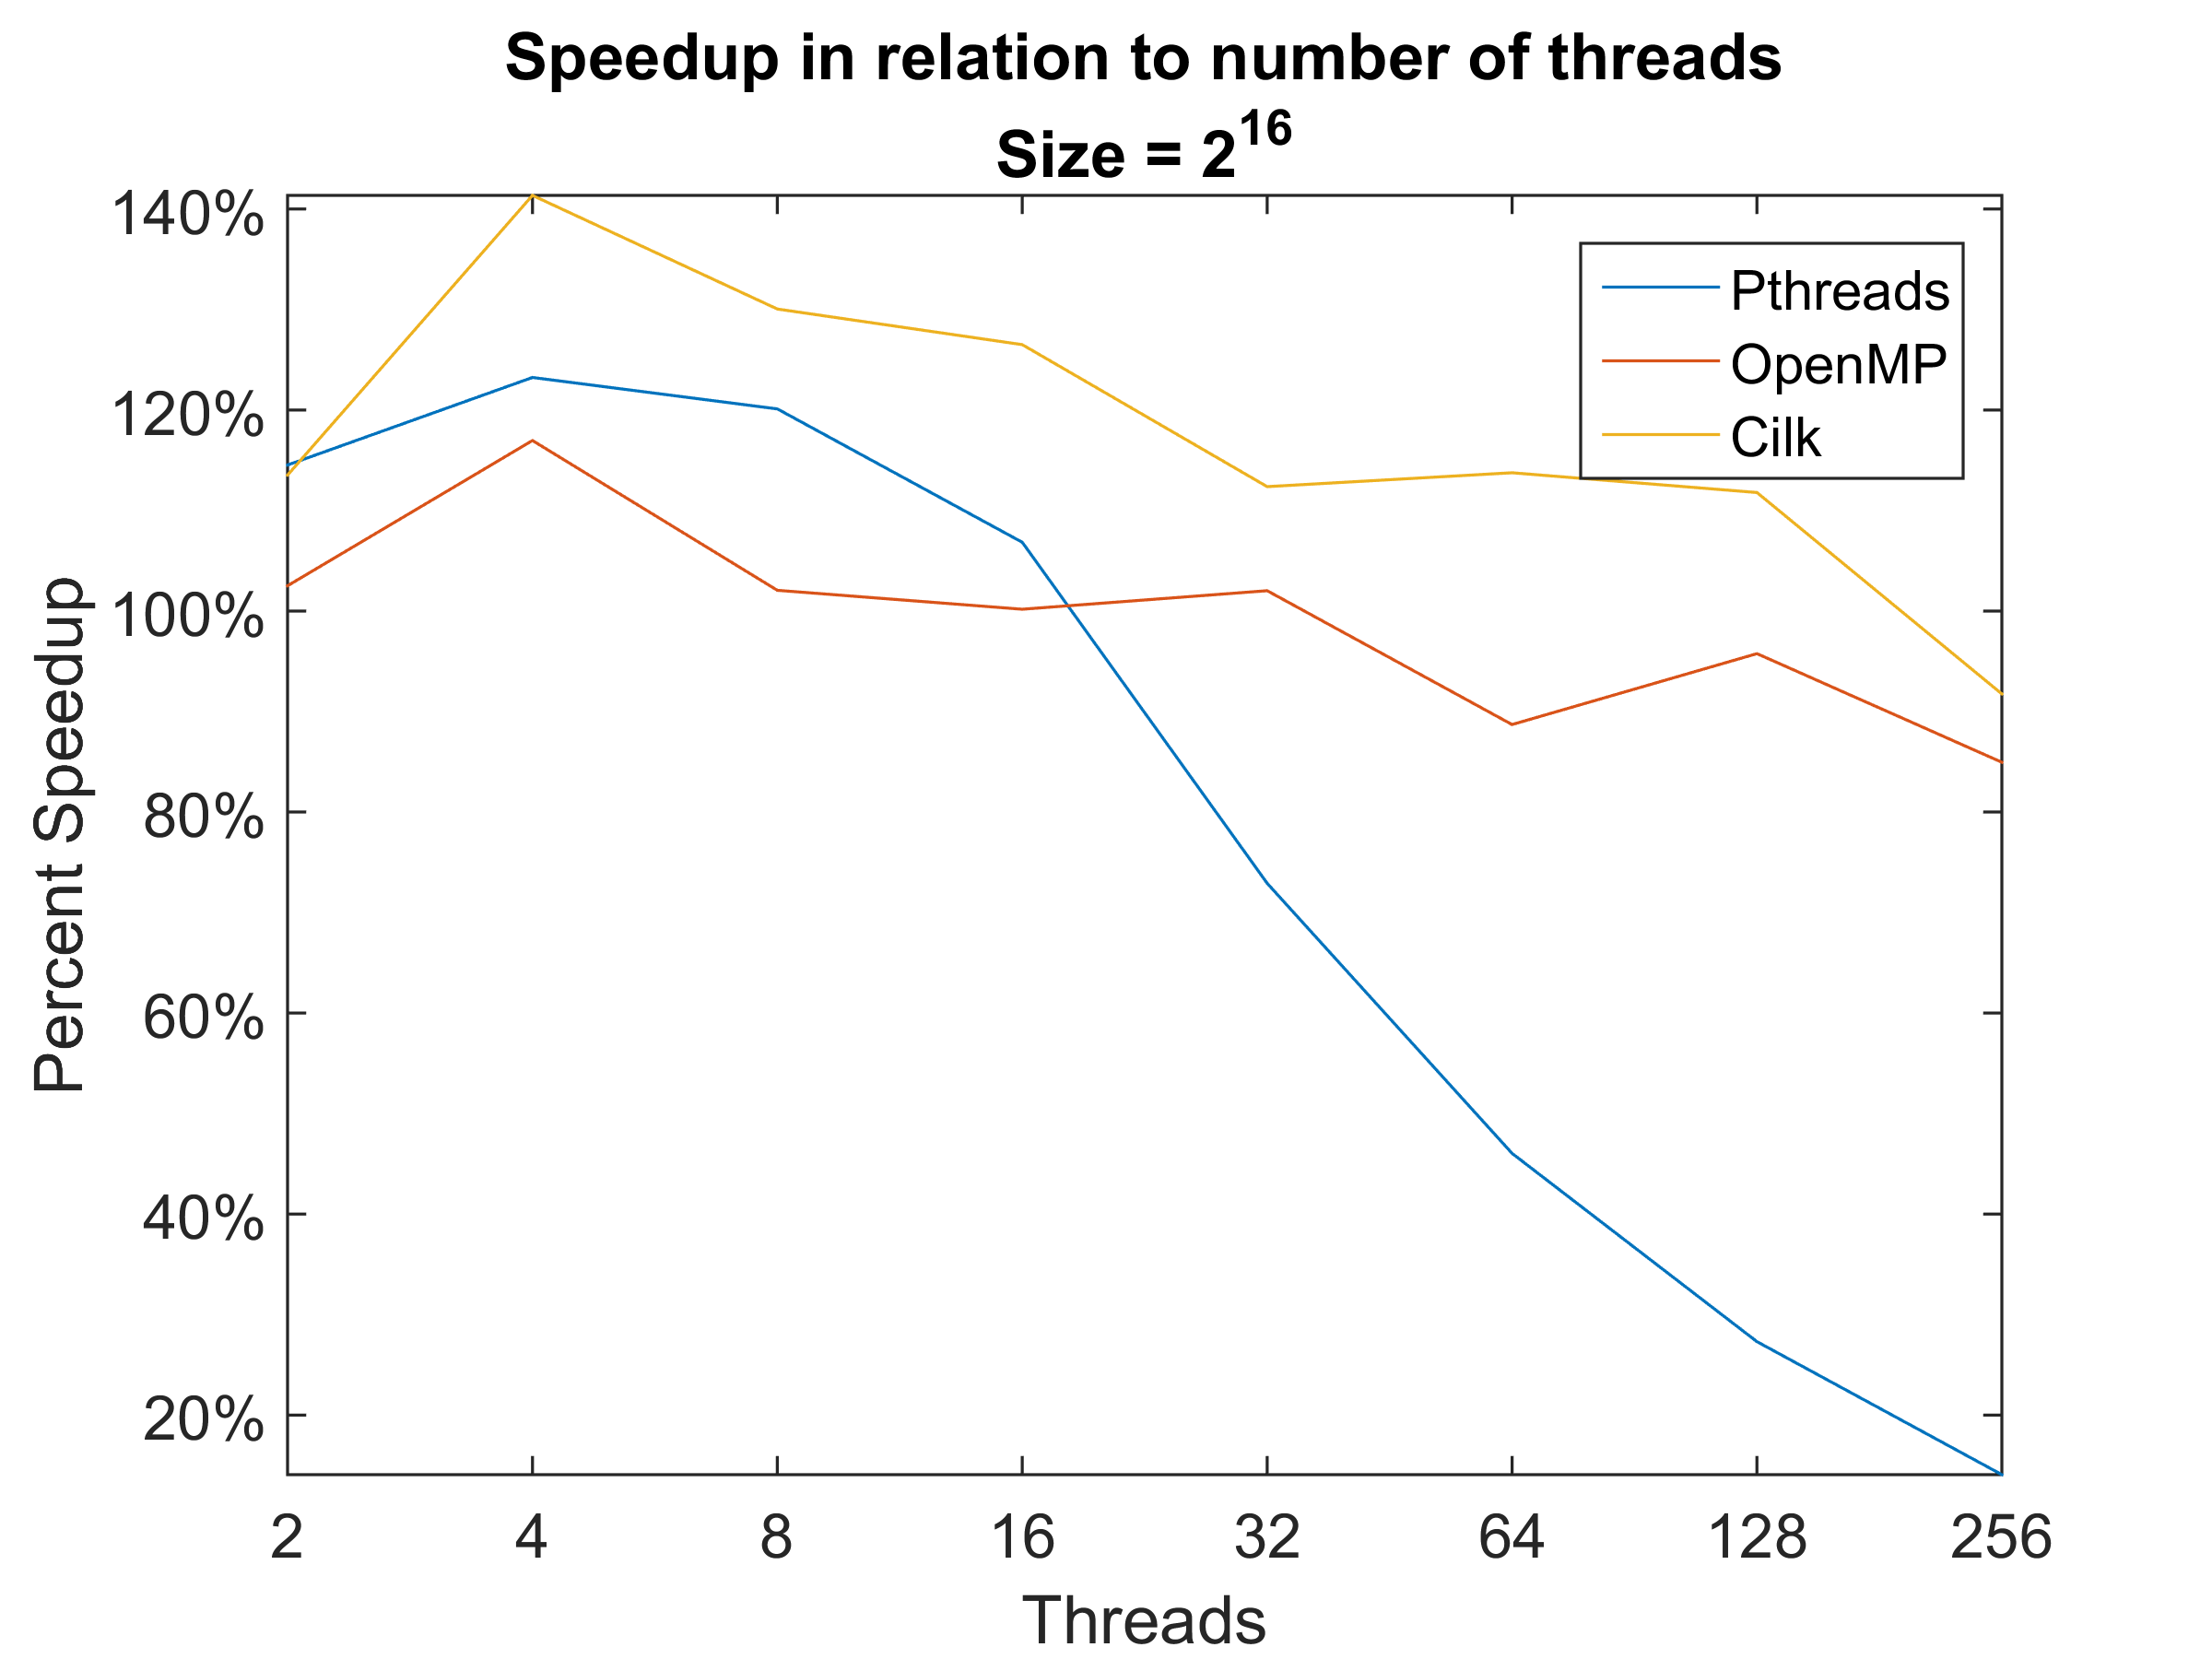
\includegraphics{figure-3.1.tikz}
		\caption{Επιτάχυνση του αλγορίθμου συναρτήσει της ανάλυσης πλέγματος ($P = 1$)}
		\label{fig:p1}
	\end{figure}
	
	Από την άλλη, το μέγεθος του προβλήματος μπορεί να επηρεάσει αρνητικά την αποδο-τικότητα του αλγορίθμου με μη προφανείς τρόπους. Για παράδειγμα στο σχήμα \ref{fig:n25}, μπορεί κανείς να δει πως ο μεγαλύτερος λόγος επιτάχυνσης είναι μικρότερος από τους προηγού-μενους. Αυτό μπορεί να οφείλεται είτε στο γεγονός ότι οι μετρήσεις μας υπόκειτω σε θόρυβο, σενάριο το οποίο δεν είναι τόσο πιθανό, καθώς οι συνθήκες είναι αρκετά ελεγχόμενες, οπότε δεν τα αποτελέσματά μας δε θα επηρεάζονταν τόσο έντονα. Ένα άλλο πιο πιθανό σενάριο, είναι ότι λόγω του αυξημένου μεγέθους του προβλήματος, οι επικοινωνίες και οι μεταφορές δεδομένων μεταξύ των διεργασιών δυσχεραίνονται και εισάγονται εμφανείς καθυστερήσεις. Για να μιλήσουμε με νούμερα, όταν έχουμε $N_Q = N_C = 2^{25}$ τότε και τα δύο σύνολα $Q, C$ ανέρχονται στα $4\, \mathrm{bytes}\cdot3\cdot2^{25}\cdot2 \approx 800\, \mathrm{Mb}$, μέγεθος το οποίο πρέπει να λαμβάνεται υπόψη, ειδικά όταν εμπλέκονται μεταφορές δεδομένων μέσω δικτυακού layer. Μάλιστα, σε πιο ρεαλιστικές συνθήκες, όπου ο αριθμός των nodes θα είναι μεγαλύτερος, με μικρότερο ppn έκαστο, το φαίνομενο αυτό θα είναι ακόμη πιο έντονο. Όμως, αυτό είναι ένα αναγκαίο κακό, καθώς οι χρόνοι εκτέλεσης του προκειμένου προβλήματος σε μεγάλα datasets είναι απαγορευτικοί. Μπορεί να μην πετυχαίνουμε την βέλτιστη θεωρητική αποδοτικότητα μέσω της παραλληλοποίησης, αλλά σε αυτά τα μεγέθη είναι μονόδρομος το διαμοιρασμένο computing.\\
	
\section{Αναφορές}
	Για την παραγωγή των διαγραμμάτων χρησιμοποιήθηκε το περιβάλλον της MATLAB, καθώς και το MATLAB script \verb|matlab2tikz|, το οποίο μπορεί να βρεθεί εδώ:\\ \url{http://www.mathworks.com/matlabcentral/fileexchange/22022-matlab2tikz-matlab2tikz}\\
	
	Για την προεπεξεργασία των δεδομένων ώστε να έρθουν σε μια πιο βολική μορφή για το MATLAB χρησιμοποιήθηκε ένα ruby script ώστε να μετατραπούν σε δομή CSV. Το script αυτό μπορεί να βρεθεί στο φάκελο \verb|results/|.\\
	
	Για την υποβολή των jobs στο Hellasgrid, χρησιμοποιήθηκε μια τροποποιημένη μορφή του ακόλουθου script:\\
	 \url{https://www.thmmy.gr/smf/index.php?topic=65374.msg1109009#msg1109009}\\
	 
	Τέλος, για διευκόλυνσή μας τροποποιήθηκε το ακόλουθο πρόγραμμα $C$, το οποίο εισάγει τη δυνατότητα χρήσης δομών τύπου vector:\\
	\url{https://www.happybearsoftware.com/implementing-a-dynamic-array}
\end{document}
